\documentclass{article}
\usepackage[T1]{fontenc}
\usepackage{lmodern}
\usepackage{graphicx}
\usepackage{amsmath,amssymb}
\usepackage[a4paper,margin=2cm]{geometry}
\usepackage[absolute,overlay]{textpos}
\setlength{\TPHorizModule}{1mm}
\setlength{\TPVertModule}{1mm}
\usepackage[indonesian]{babel}
\usepackage{hyperref}
\setlength{\emergencystretch}{2em}
\title{16-Algoritma-kripto-knapsack-2026}
\author{pdf\_ppt\_to\_latex}
\date{}

\begin{document}

% --- unit llm 1 ---
% === Halaman 1 (llm) ===

\begin{center}
Bahan kuliah IF4020 Kriptografi

{\huge \color{red} Algoritma Kriptografi Knapsack}
{\Large \color{red} (Merkle-Hellman cryptosystem)}

\vspace{20mm}

Oleh: Rinaldi M

\vspace{10mm}

Program Studi Teknik Informatika\\
Sekolah Teknik Elektro dan Informatika\\
Institut Teknologi Bandung\\
2026
\end{center}

\newpage

% --- unit llm 2 ---
% === Halaman 2 (llm) ===

\section*{Algoritma Kriptografi Knapsack}

\begin{itemize}
    \item Merupakan salah satu algoritma kriptografi kunci-publik awal yang ditemukan oleh Ralph Merkle dan Martin Hellman pada 1978.
    \item Disebut juga algoritma Merkle-Hellman
\end{itemize}

\vspace{10mm}

\begin{center}
    Merkle, Hellman, dan Diffie
\end{center}

% deskripsi: Foto hitam putih tiga tokoh kriptografi: Ralph Merkle, Martin Hellman, dan Whitfield Diffie.
% bbox normalisasi: [0.2550, 0.4660, 0.6920, 0.9050]
\begin{textblock*}{91.77mm}(53.55mm,138.40mm)
\noindent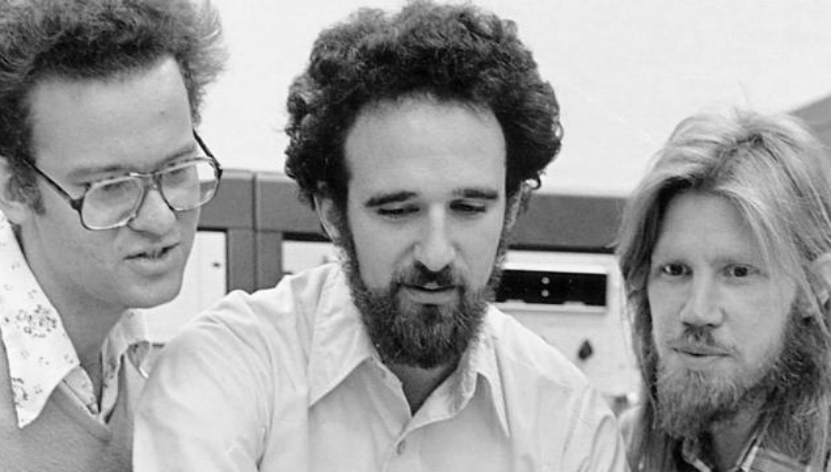
\includegraphics[width=91.77mm,height=130.38mm]{images/llm/page_002_img_01.png}%
\end{textblock*}

\newpage

% --- unit llm 3 ---
% === Halaman 3 (llm) ===

\vspace{112.86mm}

\begin{itemize}
    \item Algoritma ini didasarkan pada persoalan \textit{Knapsack Problem}:
\end{itemize}

\vspace{20mm}

Diberikan bobot \textit{knapsack} adalah $M$. Diketahui $n$ buah objek yang masing-masing bobotnya adalah $w_1, w_2, ..., w_n$. Tentukan nilai $b_i$ sedemikian sehingga

\[ M = b_1w_1 + b_2w_2 + ... + b_nw_n \eqno(1) \]

yang dalam hal ini, $b_i$ bernilai 0 atau 1. Jika $b_i = 1$, berarti objek $i$ dimasukkan ke dalam \textit{knapsack}, sebaliknya jika $b_i = 0$, objek $i$ tidak dimasukkan.

% deskripsi: Ilustrasi Knapsack Problem yang menunjukkan tas ransel dengan kapasitas 15 kg dan beberapa objek kotak dengan label harga ($) dan berat (kg) yang berbeda-beda.
% bbox normalisasi: [0.7400, 0.0200, 0.9800, 0.4000]
\begin{textblock*}{50.40mm}(155.40mm,5.94mm)
\noindent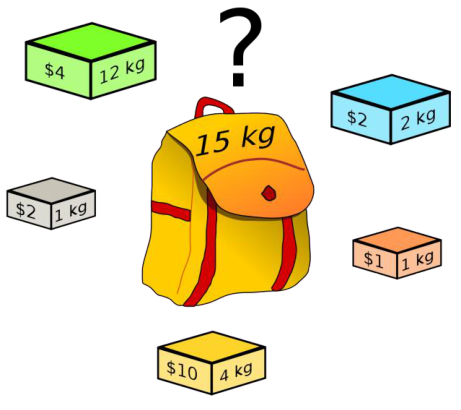
\includegraphics[width=50.40mm,height=112.86mm]{images/llm/page_003_img_01.png}%
\end{textblock*}

\newpage

% --- unit llm 4 ---
% === Halaman 4 (llm) ===

\begin{itemize}
    \item Dalam teori algoritma, persoalan \textit{knapsack} termasuk ke dalam kelompok \textit{NP-complete}.
    \item Persoalan yang termasuk \textit{NP-complete} tidak dapat dipecahkan dalam orde waktu polinomial.
    \item Ide dasar dari algoritma kriptografi \textit{knapsack} adalah mengkodekan pesan sebagai rangkaian solusi dari persoalan \textit{knapsack}.
    \item Setiap bobot $w_i$ di dalam persoalan \textit{knapsack} merupakan kunci rahasia, sedangkan bit-bit plainteks menyatakan $b_i$.
\end{itemize}

\newpage

% --- unit llm 5 ---
% === Halaman 5 (llm) ===

\textbf{Contoh 1:} Misalkan $n = 6$ dan $w_1 = 1$, $w_2 = 5$, $w_3 = 6$, $w_4 = 11$, $w_5 = 14$, dan $w_6 = 20$.

\textbf{Plainteks:} $\color{red}{1110010101100000000011000}$

Plainteks dibagi menjadi blok yang panjangnya 6, kemudian setiap bit di dalam blok dikalikan dengan $w_i$ yang berkoresponden sesuai dengan persamaan (1):

\begin{align*}$
\text{Blok plainteks ke-1} & : 111001 \\ 
\text{Kriptogram} & : (1 \times 1) + (1 \times 5) + (1 \times 6) + (0 \times 11) + (0 \times 14) + (1 \times 20) = 32 \\
\\
\text{Blok plainteks ke-2} & : 010110 \\ 
\text{Kriptogram} & : (1 \times 5) + (1 \times 11) + (1 \times 14) = 30 \\
\\
\text{Blok plainteks ke-3} & : 000000 \\ 
\text{Kriptogram} & : 0 \\
\\
\text{Blok plainteks ke-4} & : 011000 \\ 
\text{Kriptogram} & : (1 \times 5) + (1 \times 6) = 11
\end{align*}

Jadi, cipherteks yang dihasilkan: $\color{red}{32 \ 30 \ 0 \ 11}$

\newpage

% --- unit llm 6 ---
% === Halaman 6 (llm) ===

\begin{itemize}
    \item Sayangnya, algoritma \textit{knapsack} sederhana di atas hanya dapat digunakan untuk enkripsi, tetapi tidak untuk dekripsi.
    \item Misalnya, jika diberikan kriptogram $= 32$, maka tentukan $b_1, b_2, ..., b_6$ sedemikian sehingga
    
    \[ 32 = b_1 + 5b_2 + 6b_3 + 11b_4 + 14b_5 + 20b_6 \eqno{(2)} \]
    
    \item Solusi persamaan (2) ini tidak dapat dipecahkan dalam orde waktu polinomial dengan semakin besarnya $n$ (dengan catatan barisan bobot tidak dalam urutan menaik).
    \item Namun, hal inilah yang dijadikan sebagai kekuatan algoritma \textit{knapsack}.
\end{itemize}

\newpage

% --- unit llm 7 ---
% === Halaman 7 (llm) ===

\section*{Superincreasing Knapsack}

\begin{itemize}
    \item \textit{Superincreasing knapsack} adalah persoalan \textit{knapsack} yang dapat dipecahkan dalam orde $O(n)$ (jadi, polinomial).
    \item Ini adalah persoalan \textit{knapsack} yang mudah sehingga tidak disukai untuk dijadikan sebagai algoritma kriptografi yang kuat.
    \item Jika senarai bobot disebut barisan \textit{superincreasing}, maka kita dapat membentuk \textit{superincreasing knapsack}.
    \item Barisan \textit{superincreasing} adalah suatu barisan di mana setiap nilai di dalam barisan lebih besar daripada jumlah semua nilai sebelumnya.
    \item Contoh: $\{1, 3, 6, 13, 27, 52\} \rightarrow$ barisan \textit{superincreasing},
    $\{1, 3, 4, 9, 15, 25\} \rightarrow$ bukan barisan \textit{superincreasing}
\end{itemize}

\newpage

% --- unit llm 8 ---
% === Halaman 8 (llm) ===

\begin{itemize}
    \item Solusi dari \textit{superincreasing knapsack} (yaitu $b_1, b_2, ..., b_n$) mudah dicari sebagai berikut (berarti sama dengan mendekripsikan cipherteks menjadi plainteks semula):
\end{itemize}

\begin{enumerate}
    \item Jumlahkan semua bobot di dalam barisan.
    \item Bandingkan bobot total dengan bobot terbesar di dalam barisan. Jika bobot terbesar lebih kecil atau sama dengan bobot total, maka ia dimasukkan ke dalam \textit{knapsack}, jika tidak, maka ia tidak dimasukkan.
    \item Kurangi bobot total dengan bobot yang telah dimasukkan, kemudian bandingkan bobot total sekarang dengan bobot terbesar selanjutnya. Demikian seterusnya sampai seluruh bobot di dalam barisan selesai dibandingkan.
    \item Jika bobot total menjadi nol, maka terdapat solusi persoalan \textit{superincreasing knapsack}, tetapi jika tidak nol, maka tidak ada solusinya.
\end{enumerate}

\newpage

% --- unit llm 9 ---
% === Halaman 9 (llm) ===

\textbf{Contoh 2}: Misalkan bobot-bobot yang membentuk barisan \textit{superincreasing} adalah $\{2, 3, 6, 13, 27, 52\}$, dan diketahui bobot \textit{knapsack} $(M) = 70$. Kita akan mencari $b_1, b_2, ..., b_6$ sedemikian sehingga

\[ 70 = 2b_1 + 3b_2 + 6b_3 + 13b_4 + 27b_5 + 52b_6 \]

Caranya sebagai berikut:

\begin{enumerate}
    \item Bandingkan $70$ dengan bobot terbesar, yaitu $52$. Karena $52 \le 70$, maka $52$ dimasukkan ke dalam \textit{knapsack}. $\rightarrow b_6 = 1$
    \item Bobot total sekarang menjadi $70 - 52 = 18$. Bandingkan $18$ dengan bobot terbesar kedua, yaitu $27$. Karena $27 > 18$, maka $27$ tidak dimasukkan ke dalam \textit{knapsack}. $\rightarrow b_5 = 0$
    \item Bandingkan $18$ dengan bobot terbesar berikutnya, yaitu $13$. Karena $13 \le 18$, maka $13$ dimasukkan ke dalam \textit{knapsack}. $\rightarrow b_4 = 1$
\end{enumerate}

\newpage

% --- unit llm 10 ---
% === Halaman 10 (llm) ===

\begin{enumerate}
\setcounter{enumi}{3}
\item Bobot total sekarang menjadi $18 - 13 = 5$.
\item Bandingkan 5 dengan bobot terbesar kedua, yaitu 6. Karena $6 > 5$, maka 6 tidak dimasukkan ke dalam \textit{knapsack}. $\rightarrow b_3 = 0$
\item Bandingkan 5 dengan bobot terbesar berikutnya, yaitu 3. Karena $3 \le 5$, maka 3 dimasukkan ke dalam \textit{knapsack}. $\rightarrow b_2 = 1$
\item Bobot total sekarang menjadi $5 - 3 = 2$.
\item Bandingkan 2 dengan bobot terbesar berikutnya, yaitu 2. Karena $2 \le 2$, maka 2 dimasukkan ke dalam \textit{knapsack}. $\rightarrow b_1 = 0$
\item Bobot total sekarang menjadi $2 - 2 = 0$.
\end{enumerate}

\newpage

% --- unit llm 11 ---
% === Halaman 11 (llm) ===

Karena bobot total tersisa = 0, maka solusi persoalan \textit{superincreasing knapsack} ditemukan. Barisan bobot yang dimasukkan ke dalam \textit{knapsack} adalah

\[ \{2, 3, -, 13, -, 52\} \]

sehingga

\[ 70 = (1 \times 2) + (1 \times 3) + (0 \times 6) + (1 \times 13) + (0 \times 27) + (1 \times 52) \]

Dengan kata lain, plainteks dari kriptogram 70 adalah \textcolor{red}{110101}.

\newpage

% --- unit llm 12 ---
% === Halaman 12 (llm) ===

\section*{Algoritma Knapsack Kunci-Publik}

\begin{itemize}
    \item Algoritma \textit{superincreasing knapsack} adalah algoritma yang lemah, karena cipherteks dapat didekripsi menjadi plainteksnya secara mudah dalam waktu lanjar.
    \item Algoritma \textit{non-superincreasing knapsack} atau \textit{normal knapsack} adalah kelompok algoritma \textit{knapsack} yang sulit (dari segi komputasi) karena membutuhkan waktu dalam orde eksponensial untuk memecahkannya.
    \item Namun, \textit{superincreasing knapsack} dapat dimodifikasi menjadi \textit{non-superincreasing knapsack} dengan menggunakan kunci publik (untuk enkripsi) dan kunci privat (untuk dekripsi).
\end{itemize}

\newpage

% --- unit llm 13 ---
% === Halaman 13 (llm) ===

\begin{itemize}
    \item Kunci publik merupakan barisan \textit{non-superincreasing} sedangkan kunci privat tetap merupakan barisan \textit{superincreasing}.
    \item Modifikasi ini ditemukan oleh Martin Hellman dan Ralph Merkle.
\end{itemize}

\newpage

% --- unit llm 14 ---
% === Halaman 14 (llm) ===

\begin{itemize}
    \item Prosedur membuat kunci publik dan kunci privat:
\end{itemize}

\begin{enumerate}
    \item Tentukan barisan \textit{superincreasing}.
    \item Kalikan setiap elemen di dalam barisan tersebut dengan $n \pmod{m}$ \\ ( Modulus $m$ seharusnya angka yang lebih besar daripada jumlah semua elemen di dalam barisan, sedangkan pengali $n$ seharusnya tidak mempunyai faktor persekutuan dengan $m$, atau $\text{PBB}(n, m) = 1$ )
    \item Hasil perkalian akan menjadi kunci publik sedangkan barisan \textit{superincreasing} semula menjadi kunci privat.
\end{enumerate}

\newpage

% --- unit llm 15 ---
% === Halaman 15 (llm) ===

\textbf{Contoh 3:} Misalkan barisan \textit{superincreasing} adalah $\{2, 3, 6, 13, 27, 52\}$, dan $m = 105$, dan $n = 31$.

Barisan \textit{non-superincreasing} (atau normal) \textit{knapsack} dihitung sbb:

\begin{align*}
2 \cdot 31 \pmod{105} &= 62 \\
3 \cdot 31 \pmod{105} &= 93 \\
6 \cdot 31 \pmod{105} &= 81 \\
13 \cdot 31 \pmod{105} &= 88 \\
27 \cdot 31 \pmod{105} &= 102 \\
52 \cdot 31 \pmod{105} &= 37
\end{align*}

Jadi, kunci publik adalah $\{62, 93, 81, 88, 102, 37\}$, sedangkan kunci privat adalah $\{2, 3, 6, 13, 27, 52\}$.

\newpage

% --- unit llm 16 ---
% === Halaman 16 (llm) ===

\section*{Enkripsi}

\begin{itemize}
    \item Enkripsi dilakukan dengan cara yang sama seperti algoritma \textit{knapsack} sebelumnya.
    \item Mula-mula plainteks dipecah menjadi blok bit yang panjangnya sama dengan kardinalitas barisan kunci publik.
    \item Kalikan setiap bit di dalam blok dengan elemen yang berkoresponden di dalam barisan kunci publik.
\end{itemize}

\newpage

% --- unit llm 17 ---
% === Halaman 17 (llm) ===

\textbf{Contoh 4:} Misalkan

\textbf{Plainteks:}\textcolor{red}{01100011010101101110}

dan kunci publik adalah hasil dari Contoh 3,

\[ \text{Kunci publik} = \{62, 93, 81, 88, 102, 37\}, \]
\[ \text{Kunci privat adalah} \{2, 3, 6, 13, 27, 52\}. \]

Plainteks dibagi menjadi blok yang panjangnya 6, kemudian setiap bit di dalam blok dikalikan dengan elemen yang berkorepsonden di dalam kunci publik:

\newpage

% --- unit llm 18 ---
% === Halaman 18 (llm) ===

Blok plainteks ke-1 : 011000 \\
Kunci publik : 62, 93, 81, 88, 102, 37 \\
Kriptogram : $(1 \times 93) + (1 \times 81) = 174$

\vspace{5mm}

Blok plainteks ke-2 : 110101 \\
Kunci publik : 62, 93, 81, 88, 102, 37 \\
Kriptogram : $(1 \times 62) + (1 \times 93) + (1 \times 88) + (1 \times 37) = 280$

\vspace{5mm}

Blok plainteks ke-3 : 101110 \\
Kunci publik : 62, 93, 81, 88, 102, 37 \\
Kriptogram : $(1 \times 62) + (1 \times 81) + (1 \times 88) + (1 \times 102) = 333$

\vspace{5mm}

Jadi, cipherteks yang dihasilkan : 174, 280, 333

\newpage

% --- unit llm 19 ---
% === Halaman 19 (llm) ===

\section*{Dekripsi}

\begin{itemize}
    \item Dekripsi dilakukan dengan menggunakan kunci privat.
    \item Mula-mula penerima pesan menghitung $n^{-1}$, yaitu balikan dari $n$ modulo $m$, sedemikian sehingga
    \[ n \cdot n^{-1} \equiv 1 \pmod{m}. \]
    \item Kalikan setiap kriptogram dengan $n^{-1}$, lalu nyatakan hasil kalinya sebagai penjumlahan elemen-elemen kunci privat untuk memperoleh plainteks dengan menggunakan algoritma pencarian solusi \textit{superincreasing knapsack}.
\end{itemize}

\newpage

% --- unit llm 20 ---
% === Halaman 20 (llm) ===

\textbf{Contoh 5:} Kita akan mendekripsikan cipherteks dari Contoh 4 dengan menggunakan kunci privat $\{2, 3, 6, 13, 27, 52\}$. Di sini, $n = 31$ dan $m = 105$. Nilai $31^{-1} \pmod{105}$ diperoleh sbb:

\[ n \cdot n^{-1} \equiv 1 \pmod{m} \rightarrow 31 \cdot n^{-1} \equiv 1 \pmod{105} \rightarrow n^{-1} = (1 + 105k)/31 \]
coba $k = 0, 1, 2, \dots$, diperoleh $n^{-1} = 61$

Cipherteks dari Contoh 4 adalah $174, 280, 333$. Hasil dekripsi:

\begin{align*}
174 \cdot 61 \pmod{105} = 9 &= \color{red}{0} \cdot 2 + \color{red}{1} \cdot 3 + \color{red}{1} \cdot 6 + \color{red}{0} \cdot 13 + \color{red}{0} \cdot 27 + \color{red}{0} \cdot 52 \rightarrow \color{red}{011000} \\
280 \cdot 61 \pmod{105} = 70 &= \color{red}{1} \cdot 2 + \color{red}{1} \cdot 3 + \color{red}{0} \cdot 6 + \color{red}{1} \cdot 13 + \color{red}{0} \cdot 27 + \color{red}{1} \cdot 52 \rightarrow \color{red}{110101} \\
333 \cdot 61 \pmod{105} = 48 &= \color{red}{1} \cdot 2 + \color{red}{0} \cdot 3 + \color{red}{1} \cdot 6 + \color{red}{1} \cdot 13 + \color{red}{1} \cdot 27 + \color{red}{0} \cdot 52 \rightarrow \color{red}{101110} 
\end{align*}

Jadi, plainteks yang dihasilkan kembali adalah:
\[ \color{red}{011000110101101110} \]

\newpage

% --- unit llm 21 ---
% === Halaman 21 (llm) ===

\section*{Implementasi Knapsack}

\begin{itemize}
    \item Ukuran cipherteks yang dihasilkan lebih besar daripada plainteksnya, karena enkripsi dapat menghasilkan kriptogram yang nilai desimalnya lebih besar daripada nilai desimal blok plainteks yang dienkripsikan.
    \item Untuk menambah kekuatan algoritma \textit{knapsack}, kunci publik maupun kunci privat seharusnya paling sedikit 250 elemen, nilai setiap elemen antara 200 sampai 400 bit panjangnya, nilai modulus antara 100 sampai 200 bit.
    \item Dengan nilai-nilai \textit{knapsack} sepanjang itu, dibutuhkan $10^{46}$ tahun untuk menemukan kunci secara \textit{brute force}, dengan asumsi satu juta percobaan setiap detik.
\end{itemize}

\newpage

% --- unit llm 22 ---
% === Halaman 22 (llm) ===

\begin{itemize}
    \item Demo Merkle-Hellman knapsack online:
    \url{https://asecuritysite.com/encryption/knapcode?val1=3%2C%205%2C%2015%2C%2025%2C%2054%2C%20110%2C%20225&val2=10&val3=439&val4=1001000110010110110011011111}
\end{itemize}

\vspace{10mm}

% deskripsi: Screenshot aplikasi web simulasi Knapsack Encryption (Merkle-Hellman Knapsack) yang menunjukkan input kunci privat, n, modulus, dan data, serta hasil perhitungan kunci publik, cipher, inverse, dan plaintext.
% bbox normalisasi: [0.0000, 0.2700, 1.0000, 0.9700]
\begin{textblock*}{210.00mm}(0.00mm,80.19mm)
\noindent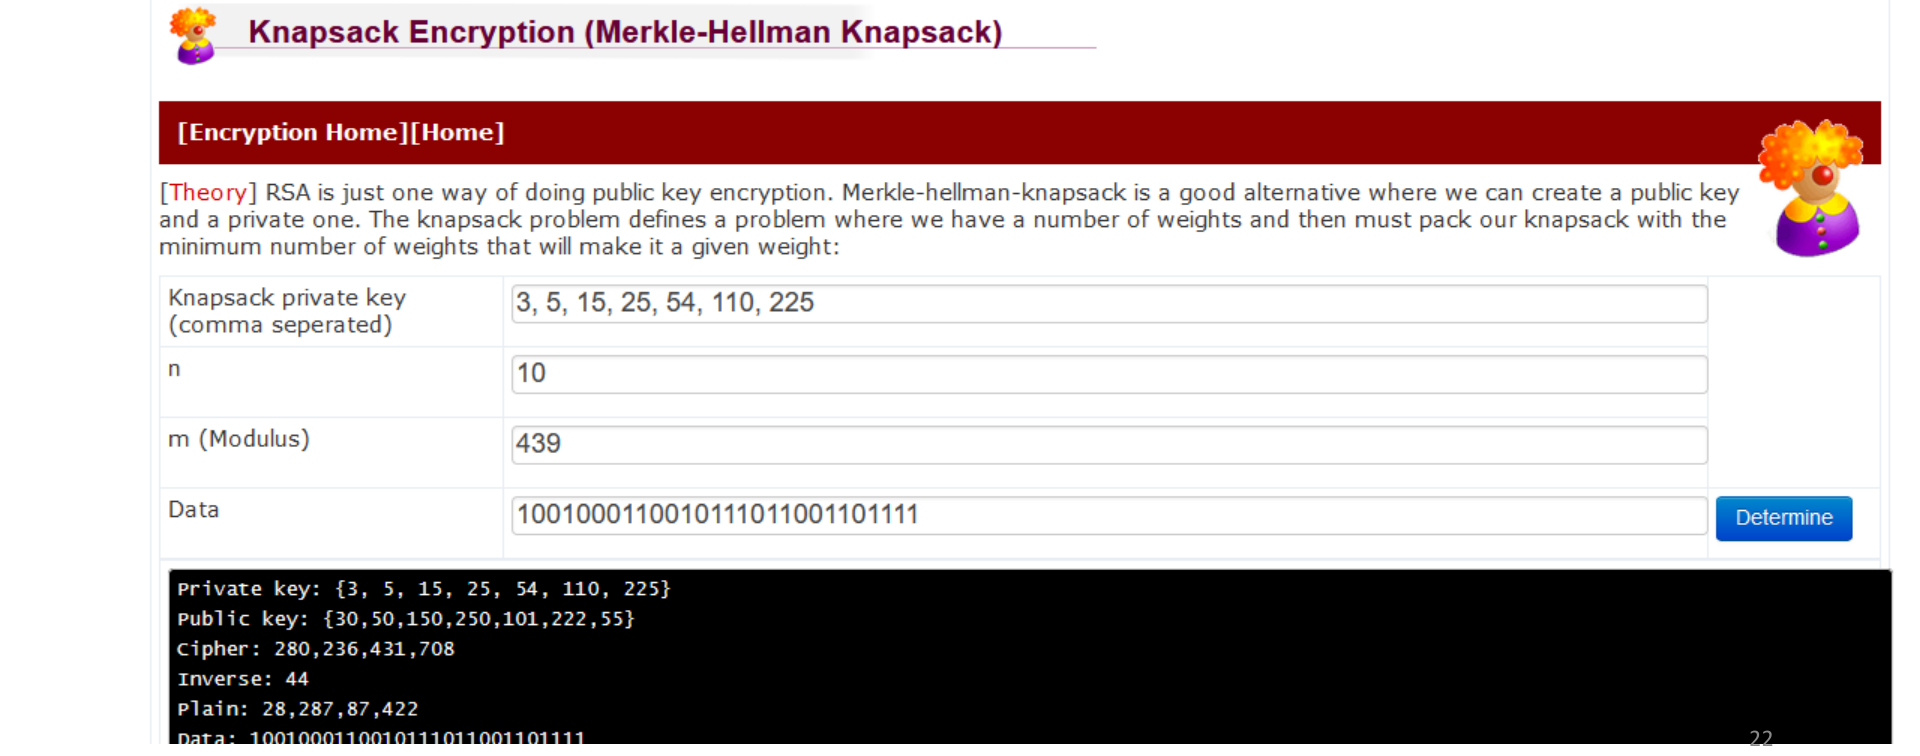
\includegraphics[width=210.00mm,height=207.90mm]{images/llm/page_022_img_01.png}%
\end{textblock*}

\newpage

% --- unit llm 23 ---
% === Halaman 23 (llm) ===

\section*{Kriptanalisis Knapsack}

\begin{itemize}
    \item Sayangnya, algoritma \textit{knapsack} dinyatakan sudah tidak aman, karena \textit{knapsack} dapat dipecahkan oleh pasangan kriptografer Adi Shamir.
    \item Shamir merumuskan transformasi yang memungkinkan mereka merekonstruksi \textit{superincreasing knapsack} dari \textit{normal knapsack} dalam waktu polynomial.
    \item Baca makalahnya: \textit{A polynomial time algorithm for breaking the basic Merkle-Hellman cryptosystem}

    (\textbf{Published in:} \href{https://doi.org/10.1145/800014.800015}{23rd Annual Symposium on Foundations of Computer Science (sfcs 1982)})
\end{itemize}

\newpage

% --- unit llm 24 ---
% === Halaman 24 (llm) ===

\begin{center}
\textbf{A POLYNOMIAL TIME ALGORITHM FOR BREAKING\\
THE BASIC MERKLE-HELLMAN CRYPTOSYSTEM}

by Adi Shamir

Applied Mathematics\
The Weizmann Institute\
Rehovot, Israel
\end{center}

\subsection*{Abstract}

The cryptographic security of the Merkle-Hellman cryptosystem has been a major open problem since 1976. In this paper we show that the basic variant of this cryptosystem, in which the elements of the public key are modular multiples of a superincreasing sequence, is breakable in polynomial time.

\subsection*{I. Introduction}

In 1976, Whitfield Diffie and Martin Hellman published their pioneering paper on public-key cryptography (Diffie and Hellman [1976]). The paper speculated that such cryptosystems exist and surveyed their potential applications, but did not describe actual implementations. In late 1976 and early 1977, the first public-key cryptosystems were discovered (see Merkle and Hellman [1978] and Rivest, Shamir and Adleman [1978]). Since then, many variants and a few new public-key cryptosystems have been proposed, but for a variety of reasons not claiming to give any ultimate answers in this sense.

An overview of the Merkle-Hellman cryptosystem can be found in Section II. In Section III we describe the cryptanalytic attack in an informal way, and in Section IV we analyze its performance. A discussion of the results appears in Section V.

\subsection*{II. The Basic Merkle-Hellman Cryptosystem}

The public encryption key in any Merkle-Hellman cryptosystem is a sequence of $n$ natural numbers $a_1, \dots, a_n$ (a typical value of $n$ is 100 and a typical size of each $a_i$ is 200 bits). To encrypt an $m$-bit cleartext $X = x_1 \dots x_m$ ($x_i \in \{0,1\}$), the sender computes a message-dependent partial sum of the $a_i$ elements:

\[ b = \sum_{i=1}^{n} x_i a_i \]

\end{document}
